\section[General k and Gadget Candidates]{General $k$ and Gadget Candidates}
\label{sec:k-extension}

The $1$-NN witness isolates the conceptual point cleanly, but it is natural to
ask whether the same separation pattern persists for larger odd values of $k$.
Our current repository contains a bounded finite search for odd-$k$ gadget
candidates, together with plots and machine-readable output. What it does not
yet contain is a fully formal lifting theorem. This section is written to make
that status transparent.

The search heuristic is motivated by a repeated-occurrence amplification idea.
If a $1$-NN witness works because one decisive nearest occurrence can be
replaced, then for odd $k$ one may hope to replicate that decisive role across
several tightly controlled occurrences so that LOO remains benign while a
targeted replace-one move still crosses the top-$k$ signed margin. The search
pipeline explores deterministic finite samples designed around this pattern.

\begin{figure}[t]
    \centering
    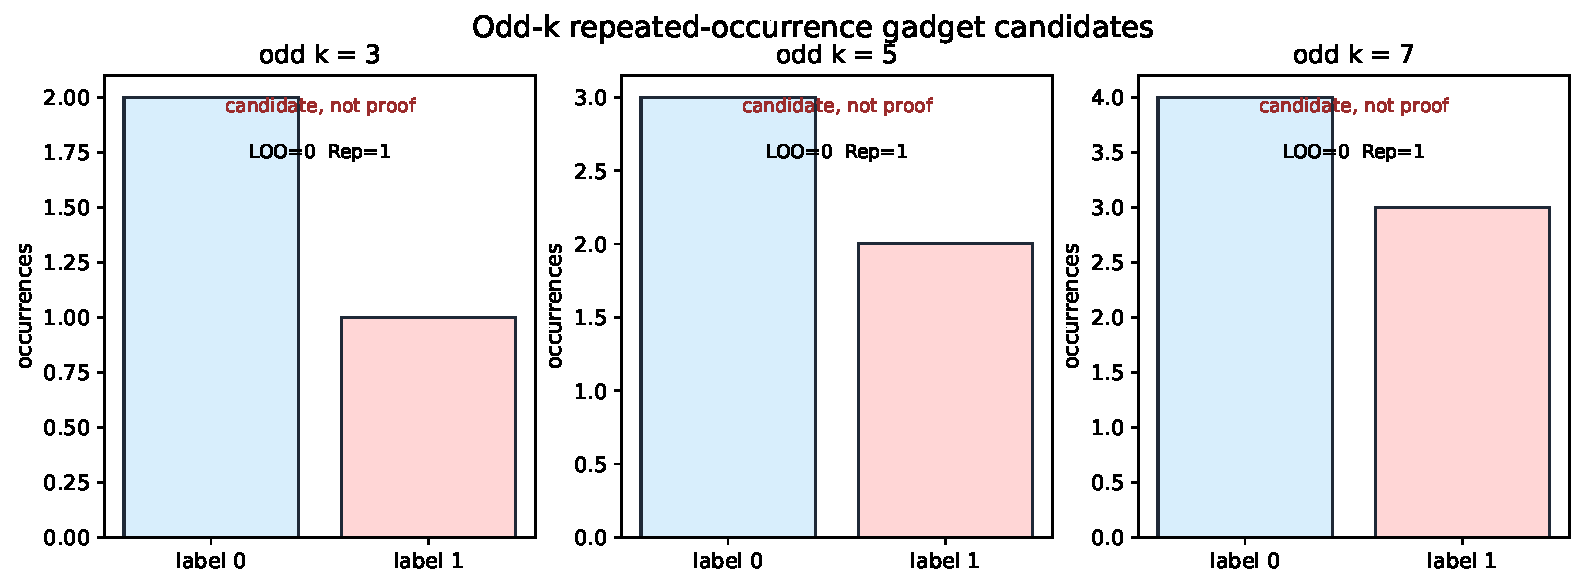
\includegraphics[width=0.86\linewidth]{outputs/figures/k_gadget_candidates.pdf}
    \caption{Representative computational candidates for odd-$k$ separations.
    These outputs are evidence for a plausible lifting pattern, not theorem
    statements.}
    \label{fig:k-gadget-candidates}
\end{figure}

\begin{table}[t]
\centering
\small
\begin{tabular}{lllllll}
\toprule
k & vertices & sample size & max LOO & max replace-one & status & script \\
\midrule
3 & 2 & 3 & 0 & 1 & computational candidate only & experiments/search\_k\_gadgets.py \\
5 & 2 & 5 & 0 & 1 & computational candidate only & experiments/search\_k\_gadgets.py \\
7 & 2 & 7 & 0 & 1 & computational candidate only & experiments/search\_k\_gadgets.py \\
\bottomrule
\end{tabular}
\caption*{\footnotesize Odd-k rows summarize one representative candidate per k and are not theorem statements.}
\end{table}


The computational record suggests the following formulation.

\begin{conjecture}[Odd-$k$ repeated-occurrence lifting]
\label{conj:odd-k-lifting}
For every odd $k \ge 1$, there exists a deterministic finite metric sample for
$k$-NN such that pointwise LOO stability holds at the designated occurrences
while pointwise replace-one instability occurs at a chosen query-label pair.
\end{conjecture}

Why not state this as a theorem? Because the present evidence is still a search
result plus a design heuristic. The candidate families for $k=3,5,7$ are real
and reproducible, but the repository does not yet contain a general proof that
the construction scales to all odd $k$, nor a proof that the searched examples
capture the true minimal combinatorics.

That said, the candidates are still scientifically useful. First, they test the
robustness of the mechanism seen in \Cref{prop:two-point-separation}: the
separation is not obviously a one-neighbor anomaly. Second, they tell us which
features seem structurally important for any future proof, namely repeated local
blocks, controlled vote margins, and deterministic tie-sensitive neighbor
ordering. Third, they warn us that an honest paper should keep a clear gradient
of claim strength: theorem, computational certificate, conjecture.

Even-$k$ appears subtler. Because the vote boundary already sits at a tied
margin, deterministic label-order tie-breaking plays a larger role, and the
search space is less cleanly explained by odd-margin amplification. We therefore
make no even-$k$ theorem claim and no impossibility claim here.
